\chapter{Methodology}

\section{TF-IDF + SVM}

	TF-IDF represent as \enquote{term frequency–inverse document frequency}. The conventional way to evaluate the semantics based on the occurrence of words and term, 
  and it also takes the occurrence of word in global context into consideration, which means the more entry the word present, less meaningful it is.

  It is simple and effective, but it still suffers from some disadvantages like data sparsity and high dimension, which may slow down the classifiers, and inability to model synonym. \\

  The SVM we conducted is LinearSVC in sklearn, which uses linear kernel. It used one-vs-rest strategy to handle the multiclass cases.
  In the other word, it generates fewer models than SVC does.
  We used default parameters. The penalty is l2, and loss function is squared hinge. 

\section{Fasttext}
	
The approach is purposed by \cite{joulin2016fasttext}. 
The structure of FastText can be considered as extension of word2vec as well, and it uses the hierarchical softmax to compute the probabilities for predefined classes. 
However, the key difference of fasttext from word2vec is that it employed bag of N-grams features. 
For example the word vector “apple” is a sum of the vectors of the N-grams “\textless ap”, “app”, ”appl”, “apple”, “apple\textgreater”, “ppl”, “pple”, “pple\textgreater”, “ple”, “ple\textgreater”, “le\textgreater”.
This approach tries to take the local word order into consideration and evaluate the partial information from spelling. It may also vectorize the rare words better, which have less neighboring words to model.
It also a countermeasure to solve the problem of bag-of-words, that the order of words is not considered. 
For example, the terms \enquote{我見你} (I see you) and \enquote{你見我}(you see me) are contributed to the same results in bag of words model.
However, in the ngrams model, the vector are average from its subset, including \enquote{我見}(I see), \enquote{我} (I)...etc, it makes it possible to distinguish the difference.

While the computation and space complexity increase, it employs the hashing trick like word2vec as well. 
The word representation is looked up through a table and finally averaged into the text representation. 
For the words absent from word embeddings, it uses subword infomation\cite{bojanowski2016enriching} to guess the meaning of the word.
Another trick applied is pruning some of the vocabulary elements. Feature selection among N-gram is very inefficient and complicated.
Here it used online parallelizable greedy approach: To check if the document is covered already, if not, add one with the highest norm.

Finally, it uses the linear classification to classify the data. The classifier called \enquote{Product quantization} uses some tricks to speed up, which utilizes compressed-domain approximate nearest neighbor search (Jegou et al., 2011) \cite{jegou2011searching}.
The compression technique approximates a real-valued vector by finding the closest vector in a predefined structured set of centroids like Figure \ref{fig:pq}.
The original PQ has been concurrently improved by Ge et al. \cite{ge2013optimized} and Norouzi \& Fleet , who learn an orthogonal transform minimizing the overall quantization loss.
The technique may sacrifice some accuracy to gain much more performance and efficiency of memory. It is proved by their experiment that with normalization, both PQ and OPQ are almost lossless with 4 subquantizers. 
We used the released build from Facebook github.

\begin{figure}[h]
    \centering
	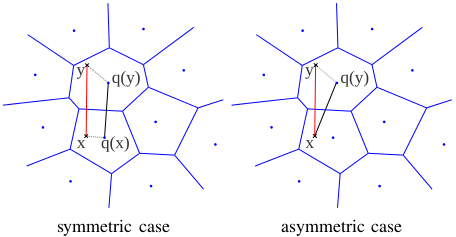
\includegraphics[width=.8\linewidth]{pq}
    \caption{Production quantization: It use predefined centroids to proximate the distance of 2 points. There are two type of PQ, symmetric and asymmetric. }
    \label{fig:pq}
\end{figure}

\begin{figure}[h]
    \centering
	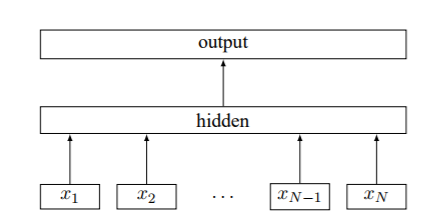
\includegraphics[width=.8\linewidth]{fasttext}
    \caption{The architecture of FastText: the image is cited from \cite{joulin2016fasttext}.}
    \label{fig:fasttext}
\end{figure}


\section{Paragraph Vector}
	
The method is purposed in \cite{PVDM}. The idea is to obtain the summary of paragraphs, sentences or documents. 
There are 2 different algorithms they purposed, which are distributed memory(DM) and distributed bag of words(DBOW). 
The DM model in figure \ref{fig:dm} is quite similar with word2vec. The difference between PVDM and word2vec is that the former contains paragraph matrix.
Every paragraph is mapped to unique vector. Figure \ref{fig:dbow} show the model architecture. DBOW is conceptually simple compared to DM model, this model store less data. 

The paragraph vectors are asked to contribute to the prediction task of the next word given many contexts sampled from the paragraph.
The contexts are fixed-length and sampled from a sliding window over the paragraphs. Therefore, DM take the sequence into consideration.

However, it ignores context words from input and forces the model to predict words randomly sampled from the paragraph in the output in DBOW model.
It is quite similar to Skip-gram in word2vec.

The author suggested that DM is consistently better in general cases, while DBOW take fewer resources. 
The author claimed it is applicable to both short sentence and long paragraph.

We use the implementation from Gensim, which support both DM and DBOW models. We use SVM with linear kernel as classifier.

\begin{figure}
\centering
\begin{subfigure}{.5\textwidth}
  \centering
  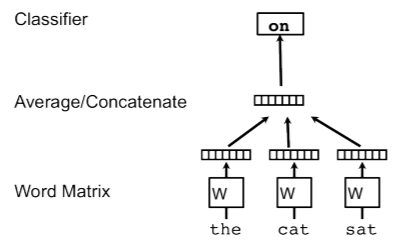
\includegraphics[width=.9\linewidth]{dm}
  \caption{distributed memory}
  \label{fig:dm}
\end{subfigure}~
\begin{subfigure}{.5\textwidth}
  \centering
  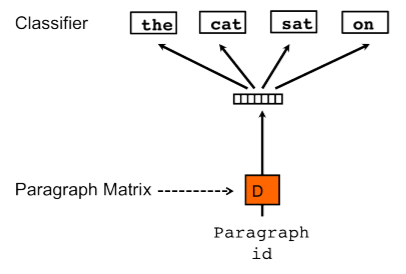
\includegraphics[width=.9\linewidth]{DBOW}
  \caption{distributed bag of words}
  \label{fig:dbow}
\end{subfigure}
\caption{Paragraph vector: the images show the difference of two models, and the images are from \cite{PVDM}.}
\label{fig:PVDM}
\end{figure}

\section{Siamese-CBOW}

The Siamese-CBOW\cite{kenter2016siamesecbow} computes sentence embeddings is to average the embeddings of its constituent words, instead of using pre-trained word embedding. It applied the concept of bag of word from word2vec. 
It used the average from the words composing the sentence and use it to evaluate the possibility to predict the sentence around. 

The architecture shows as Figure \ref{fig:siamese}. As it indicated, the word embeddings are optimized directly for averaging.
A supervised training criterion by predicting sentences occurring next to each other in the training data.
Cosine similarities are used to compute the proximity of sentences.
Softmax is applied in the last layer to produce the final probability distribution.

The authors also evaluated the effect of the hyperparameters. The number of negative sampling yield limited loss, and the higher dimension is preferred to generate better result.

We used the implementation (https://bitbucket.org/TomKenter/siamese-cbow/overview) from the authors.
We made it able to run in python3 for better compatibility with unicode.

\begin{figure}[h]
    \centering
	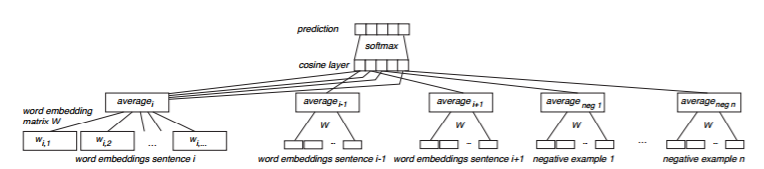
\includegraphics[width=.9\linewidth]{siamesecbow}
    \caption{The architecture of Siamese-CBOW, the image is from original paper\cite{kenter2016siamesecbow}.}
    \label{fig:siamese}
\end{figure}
